\documentclass[UTF8]{ctexart}
    \title{\huge MNIST实验报告}
    \author{\large 2015011308 计53 唐适之}
    \date{}
    \usepackage[top=1in, bottom=1in, left=1.25in, right=1.25in]{geometry}
    \usepackage{enumitem}
    \usepackage{graphicx}
    \usepackage{caption}
    \usepackage{float}
    \renewcommand{\figurename}{Figure}
    \renewcommand{\contentsname}{Contents}

\begin{document}

    \maketitle

    \section{实验结果}

        本次实验中,我使用CNN模型在Kaggle上(用户tsz2015011308)达到了0.99514正确率,提交12次;使用MLP模型达到了0.98129正确率,提交2次;共计提交14次。CNN模型和MLP模型最好的一次提交各见如下截图。

    \begin{figure}[htp]
            \centering
            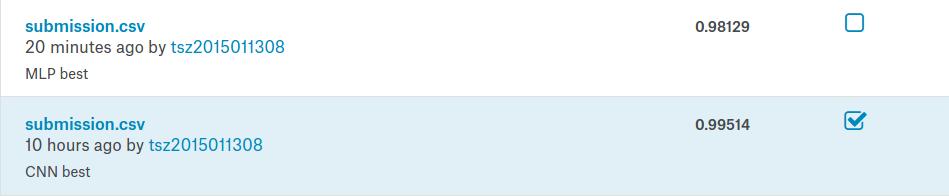
\includegraphics[width=\textwidth]{images/Screenshot.png}
            \caption{CNN和MLP最佳提交的截图}
        \end{figure}

    \section{模型及训练方法}

        \subsection{网络的拓扑结构}
            对于CNN,输入经两个卷积池化层、一个大小为1024的全连接隐层后,由一个线性输出层输出。由于是分类问题,采用softmax交叉熵损失函数。

            每个卷积池化层包含一个5*5卷积层和一个2*2最大值池化层。第一个卷积层将输入从1个分量(灰度)变为32个分量,第二个卷积层将32个分量变为64个分量。实验中没有观察到显著的过拟合现象,说明网络没有过于复杂,卷积核大小与分量数可以进一步提高。但实验表明,扩大卷积核与提高分量数对正确率没有显著影响,但大大减慢了收敛速度。为兼顾正确率与训练效率,最终选择此值。

            为了避免过拟合,在两个卷积池化层和全连接隐层后,在训练时分别以0.25的概率dropout分量,而在测试和验证时不进行dropout。

            激活函数选用elu而不是relu,因为relu在$x<0$时斜率为0,造成无法继续梯度下降。实验表明,用elu取代relu后,一开始收敛更慢,但当验证集上正确率大于0.99后,验证集上的正确率随着训练的进行波动更大,可以推测认为elu使梯度下降时各参数变化更“活跃”。

            对于MLP,网络只包含两个大小为1024的隐层、一个线性输出层,采用softmax交叉熵损失函数。其他参数同上。实验表明,隐层大小为1024依然不足(见以下“训练方法”一节),但由于MLP中每个结点都要与前一层的所有结点相连,参数量非常庞大,以至于硬件条件不允许我继续增大网络规模。

        \subsection{训练方法}
            无论CNN还是MLP,都选用了AdamOptimizer作为优化器。训练时,先用$10^{-4}$的学习率训练$5*10^4$轮,再用$10^{-5}$的学习率训练$7*10^5$轮。首先使用较大的学习率有利于快速到达最优值附近,并避免陷入局部最优,接着使用较小学习率有利于在最优值附近微调。实验表明,$10^{-5}$已是最小的可以接受的学习率,若继续降低学习率,则会陷入局部最优,表现为正确率不再显著变化。实际训练时,为了便于调整学习率,一次训练中我分多次运行程序,并对每次训练的每次运行编写配置文件。学习率写在配置文件中,程序以配置文件中的参数进行学习。

            Kaggle提供的训练集一共42000个样本,我将前5000个样本用作验证集,不参与训练,后37000个样本作为真正的训练集。实验发现,验证集偏小,在验证集上正确率达99.3以上时,验证集上的正确率的变化不能准确反映实际测试集上的变化:虽然验证集上正确率在波动,但测试集上的实际正确率随着训练轮数的增加仍在提高。但为了避免训练集过小,我没有继续增大验证集。

            每轮学习时,使用大小为50的batch进行学习。为使batch的抽样更加均匀,我并非每次学习时都独立地从训练集中抽取batch,而是先将训练集里每50个样本划分为一组,然后遍历这些组进行学习。每进行$10^5$次学习,重新进行一次划分。

            训练CNN时,我对输入图像进行了预处理。每张图像进行20度以内的随机旋转,边长15\%以内的随机平移(x、y两个方向),和以$[0.8,1.2]$区间内放大倍率的随机缩放。这样相当于产生了许多新的训练样本,扩大了训练集大小。实验表明,此举显著提高了正确率,使测试集上正确率从0.993增加到0.995。但是,在MLP模型上无法使用这样的预处理:由于预处理后训练样本更“难”了,甚至可能超出了测试集的难度,MLP也不具有CNN善于处理平移图像的优点,两个1024大小的全连接层并不足以处理它,实际表现为训练集上的正确率不收敛,然而由于MLP模型中参数太多,硬件条件又不允许继续扩大网络,故无法应用此项预处理。另外,由于预处理是在CPU上运算的,此举使训练速度显著降低。

    \section{程序运行方法}

        请参见README.md。


\end{document}

